\documentclass[10pt,a4paper]{article}

\oddsidemargin 0pt
\evensidemargin 20pt
\marginparwidth 29pt
\textwidth 470pt

\textheight 720pt
\topmargin -40pt

\usepackage[latin1]{inputenc}
\usepackage{amsmath}
\usepackage{amsfonts}
\usepackage{amssymb}
\usepackage{graphicx} 
\usepackage{longtable}
\usepackage{subcaption}
\usepackage{wrapfig}

%============================================================================================
\newtheorem{remark}{Remark}
\newtheorem{definition}{Definition}
\newtheorem{notation}{Notation}
\newtheorem{issue}{Issue}
\newtheorem{question}{Question}
\newtheorem{assumption}{Assumption}
\newtheorem{example}{Example}

%============================================================================================
\title{Flow reroute problem}
\author{Author}

\begin{document}
\maketitle

\section{Thoughts on using CMS for rerouting control: problem dimensions}

We begin by stating the various dimensions of the problem.
\begin{itemize}
\item Problem types (scenarios) we want to do control to relieve
	\begin{itemize}
	\item recurring congestion
	\item congestion due to pre-planned events and related demand
	\item congestion due to incidents
	\end{itemize}
	Relieving congestion due to incidents requires an online model, and detection of incidents. For pre-planned events and recurring congestion, we need to use estimates (e.g. historical) of demands to do the forward simulation.
\item Control objective
	\begin{itemize}
	\item System optimal (SO) flows (unlikely without incentives)
	\item User optimal (UE), Nash equilibrium
	\end{itemize}
	If we want to do control based solely on CMS, then if we simply display real time information (and only give true information), we will push the system towards a Nash equilibrium (UE). This can still be interesting if the uncontrolled state is worse than Nash. If we want to do better than Nash, then we need to think about what kind of information to display (while still being truthful).
\item On-line Vs. off-line

	We need historical estimates in all cases to be able to forward simulate the system. For on-line control we additionally need real time measurements.
	
\item Compliance rate
	\begin{itemize}
	\item Full compliance
	\item Partial compliance
	\end{itemize}
\item Control mechanism
	\begin{itemize}
	\item Phone app
	\item Changeable message signs (CMS)
	\end{itemize}
	If we use a phone app, we will have better estimates (OD demands), and more refined control (control can be adapted to individuals). If we use CMS, the same message is displayed to everyone.
	
\item Control response model
	\begin{itemize}
	\item Explicit control of vehicles to a given route (Incentive for taking a new route. Most likely this will require a phone app)
	\item Control via information (CMS)
	\item Implicit control via prodding (CMS)
	\end{itemize}	
	
\item Buffer model\footnote{See section~\ref{sec:FIFO} on the boundary FIFO problem for details}
	\begin{itemize}
	\item One large buffer (most relaxed FIFO)
	\item Many cell-sized buffers with one large last buffer
	\item One cell sized buffer with a feeder queue
	\end{itemize}
\item Input data: Historical and Real-time
	\begin{itemize}
	\item Aggregate flows across all links only (most likely)
	\item Aggregate flows across all links plus OD for controllable flow (possible with phone based control)
	\item Full OD data (pipe dream)
	\end{itemize}	
	We will most likely need an estimate of the OD for the controllable flow for the problem to be meaningful.
\item Route information encoding
	\begin{itemize}
	\item Path-based
	\item Split ratio based
	\end{itemize}
	Path-based information gives a cleaner formulation, but requires more storage, and more input data (OD estimates). Depending on the network structure, a path-based formulation may be OK (e.g. parallel network)
\item controllable OD estimation via boundary flows (behavior model)
	\begin{itemize}
	\item Online OD estimation via response to control
	\item Offline OD estimation via some historical model
	\end{itemize}	
	Estimate the OD demands for the controllable flow.
\item Network types
From most to least restrictive. The less restrictive, the more data we need.
	\begin{itemize}
	\item Single destination for controllable flow with no off and on ramps
	\item Single destination for controllable flow with either on or off ramps (can recover controllable flow)
	\item Single destination for controllable flow with on and off ramps
	\item Multiple destinations for controllable flow
	\end{itemize}
	In the single destination with no on-ramps or no off-ramps, it is sufficient to know the total flux demand and the split ratios. If we have both on-ramps and off-ramps, we additionally need an estimate of the OD demand for the controllable flow.
\item  Limitations of CMS control
	\begin{itemize}
	\item Most probably a binary controller, but we might be able to increase the granularity of control via the strength of the wording. 
	\item No Lagrangian data as in the phone based control approach.
	\end{itemize}
	We may need to abstract the control for now, by assuming that we control a split ratio at a given junction, and solve for the optimal split ratio. Then we map the optimal control strategy to an actual message to display, but that is a separate problem.
\end{itemize}




\section{Potential models with limited input data}
Let there exist a particular origin-destination pair $o-d$ with a
CMS near $o$. There are two paths that can be taken to go between
$o$ and $d$, and the CMS will post a message addressed to those
traveling $o-d$ to take route 1 over 2, with some percentage of those drivers complying. For simplicity, we assume instead that our control is a split
ratio $\beta$ for the $o-d$ drivers at the point of the CMS.

In addition, there an arbitrary
number of additional sources and sinks, but the CMS only targets $o-d$.
The additional sources and sinks may have viable paths through both
$o$ and $d$, complicating the determination of demand between $o-d$
specifically. The Eulerian flow is known over each link in the network,
over all discrete time steps.

We cannot determine which flows belong to $o-d$ drivers versus all
others from this problem setup due to the non-uniqueness of OD-estimation
problem. But if we assume we know the path flows of just taking $o-d$,
then source flows and split ratios may be determined for the other
OD's. From this assumption of data (path flows for $o-d$, source
flows and split ratios for all others), one can use the Piccoli class-based
forward simulation framework as the flow model, where the classes
are controllable $o-d$ flows and uncontrollable flows from all other
OD pairs. This is illustrated in Figure~\ref{fig:Diagram-of-network}.
\begin{wrapfigure}{r}{0.2\textwidth}
\begin{centering}
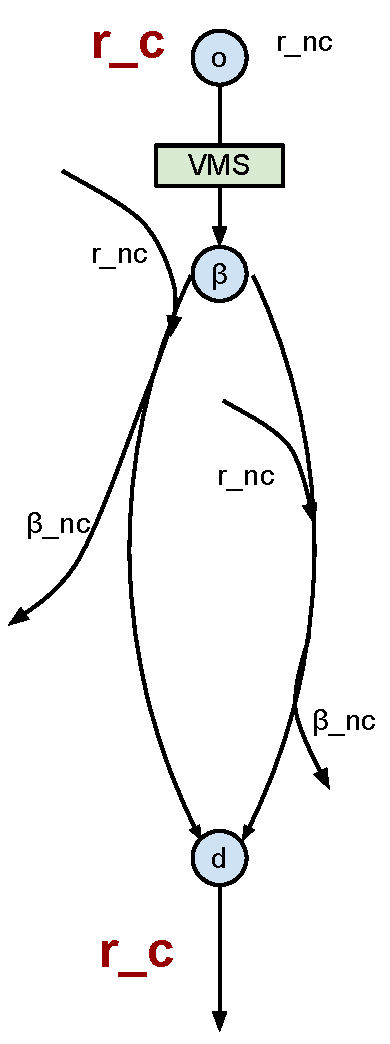
\includegraphics[scale=0.4]{NetworkForCMS}
\par\end{centering}

\caption{Diagram of network under consideration\label{fig:Diagram-of-network}. $r_c, r_{nc}$ are the flows in for controllable and non-controllable drivers. $\beta_{nc}$ are the estimated split ratios for the non-controllable, which can be determined after estimating initial controllable flows on the left and right paths.}
\end{wrapfigure}


One special case of this set of assumptions is rerouting drivers not
attending a popular event, while those attending have no rerouting
options.

One approach is to determine an upper and lower bound on the demands
on routes 1 and 2 for $o-d$. Then we take a robust optimization approach
to create an optimal split-ratio policy $\beta^{*}$ for the worst
case \emph{actual} demand on $o-d$. It is unclear how robust optimization
exactly fits within the adjoint framework, but there is previous work
in this area.

Another approach seeks to \emph{learn} the $o-d$ demands at the CMS
location from a feedback-loop approach. After witnessing how the split
ratio at the CMS changes due to some displayed split ratio, one can
estimate the population of drivers that responded to the message from
all drivers on the network.

Both of these approaches attempt to deal with the fact that we do
not have enough information to do rerouting at the CMS and still guarantee
that the original demand profiles would be satisfied. Any approach
that seeks to do rerouting on Eulerian data would have to embrace
such methods in some form.


\section{Solving the FIFO problem at the boundary of the network}
\label{sec:FIFO}
In the multi-class case of the discretized LWR models (as in Piccoli) the FIFO assumption is typically satisfied at the cell level. This is not full FIFO at the individual car level, but an accepted approximation of FIFO. In our buffer based boundary cell model, the FIFO assumption is further relaxed as the buffer can accumulate a large number of vehicles over time when the boundary is congested and the FIFO condition will only apply in this aggregate sense. To alleviate this problem, we need to keep track of the ratios of controllable and non-controllable vehicles that enter the boundary at a more granular level. The solution that would be equivalent to what happens within the network would be to have multiple buffers of the same size as a single cell and move flow forward through the buffers as the first buffer empties into the network. There need to be enough buffers to handle the maximum possible queue length at the boundary. A more precise way to follow the ratios would be to have a single buffer that is the same size as a cell and then keep an overflow queue for vehicles that can not enter the buffer. This queue will keep all the entering vehicles in order and feed them into the buffer as space opens up. The vehicle ratio at the buffer will be updated accordingly as new vehicles enter it. We require $\log_{2}$(max\_queue\_length) bits of storage at each boundary to store this information, but this should be a relatively small and manageable number. Modifications will be needed to have the derivative make sense in the adjoint formulation.

% \section{Outstanding issues}
% \subsection{Problems with time-varying $\beta$}


% \begin{itemize}
% \item 
% \end{itemize}


%-----------------------------------------------------------------------------------------------------------------------------------------------------------------
\bibliographystyle{plain}
\bibliography{jackbibdontedit}

\end{document}